\documentclass[10pt]{article}

\usepackage[letterpaper, left=1in, right=1in, top=1in, bottom=1in]{geometry}
\usepackage{amssymb, longtable, booktabs}
\usepackage{minted, color, setspace}
\usepackage{titlesec}
\usepackage{graphicx, subfigure}
\usepackage{hyperref, url}

\hypersetup{%
    pdfsubject={LaTeX Document},
    colorlinks=true,   % false: boxed links; true: colored links
    linkcolor=blue,    % color of internal links
    citecolor=blue,    % color of links to bibliography
    urlcolor=blue,     % color of external links
    unicode=false      % non-Latin characters in Acrobat's bookmarks
}

\makeatletter
\def\maketitle{\begin{center}{\bfseries \Large ECE-C353 Systems Programming \\ \@title} \end{center}\vspace{10pt}}
\makeatother

\titleformat{\section}{\normalfont\bfseries}{}{5pt}{}
\titlespacing{\section}{-5pt}{12pt plus 4pt minus 2pt}{0pt plus 2pt minus 2pt}

\setlength{\parindent}{0pt}
\setlength{\parskip}{8pt}

\definecolor{lightgray}{rgb}{0.95,0.95,0.95}

\newcommand{\ctrl}[1]{\texttt{\textbf{\string^#1}}}
\newcommand{\checkbox}[0]{\makebox[0pt][l]{$\square$}\raisebox{.15ex}{\hspace{0.1em}}}

\title{Project 2 -- Basic Shell Part 2: Job Control}

\begin{document}
\maketitle

\vspace{-24pt}

\begin{center}
\vspace{12pt}
\textbf{Due Thursday, Mar 8th \emph{before} midnight.}
\end{center}

\begin{center}
    \texttt{START THIS PROJECT EARLY}

    \texttt{READ THIS ENTIRE DOCUMENT\\(TWICE)}
\end{center}

\section{The Big Idea}

In this assignment you will be building upon the basic shell you
developed in Project 1.  Specifically, we will be focusing on
\textbf{Process Groups}, \textbf{Signals}, and \textbf{Signal Handlers}
in order to implement a standard job control system similar to the ones
found in most shells.  In this context, a \emph{job} is the execution of
a single command line entry.  For example:

\begin{minted}[bgcolor=lightgray]{text}
   $ ls -l
\end{minted}
is a single job consisting of one process.  Likewise,

\begin{minted}[bgcolor=lightgray]{text}
   $ ls -l | grep .c
\end{minted}
is a single job consisting of two processes.

\vspace{12pt}

Upon successful completion of this project, your shell will have the
following additional functionality:

\begin{itemize}
    \item You will be able to check the status of jobs with the new built-in \texttt{jobs} command

    \item You will be able to suspend the foreground job by hitting \texttt{Ctrl+z}

\begin{minted}[bgcolor=lightgray]{text}
$ sleep 100
^Z[0] + suspended       sleep 100
$ jobs
[0] + stopped   sleep 100
$
\end{minted}

    \item You will be able to continue a stopped job in the background using the new \texttt{bg} command:

\begin{minted}[bgcolor=lightgray]{text}
$ jobs
[0] + stopped   sleep 100
[1] + stopped   sleep 500
$ bg %1
[1] + continued sleep 500
$ jobs
[0] + stopped   sleep 100
[1] + running   sleep 500
$
\end{minted}

    \item You will be able to start a job in the background by ending a
        command with the ampersand (\texttt{\&}) character.  Doing this
        causes the shell to display the job number and the involved process
        IDs separated by spaces:

\begin{minted}[bgcolor=lightgray]{text}
$ frame_grabber cam0 | encode -o awesome_meme.mp4 &
[0] 3626 3627
$ jobs
[0] + running   frame_grabber cam0 | encode -o awesome_meme.mp4 &
$
\end{minted}

\pagebreak

    \item You will be able to move a background or stopped job to the
        foreground using the new built-in \texttt{fg} command:

\begin{minted}[bgcolor=lightgray]{text}
$ jobs
[0] + running   frame_grabber cam0 | encode -o awesome_meme.mp4 &
$ fg %0
encoding frame 42239282 [OK]
encoding frame 42239283 [OK]
encoding frame 42239284 [OK]
encoding frame 42239285 [OK]
encoding frame 42239286 [OK]^Z
[0] + suspended      frame_grabber cam0 | encode -o awesome_mem.mp4 &
$
\end{minted}

    \item You will also be able to kill all processes associated with a
        job using the new built-in \texttt{kill} command:

\begin{minted}[bgcolor=lightgray]{text}
$ jobs
[0] + running   frame_grabber cam0 | encode -o awesome_meme.mp4 &
$ kill %0
[0] + done     frame_grabber cam0 | encode -o awesome_meme.mp4 &
$
\end{minted}

\end{itemize}

\vspace{48pt}

Please keep in mind that you will most probably need the full time
allotted for this assignment.  There are many asynchronous things going
on between the shell and the jobs it manages, which are being
coordinated by various signals.  Give yourself enough time to get things
wrong, figure out what is happening, and correct your code.


\pagebreak

\section{Using Process Groups}

\emph{Process Groups} are, as the name would imply, a group of
processes.  Each process group has a \emph{process group ID (PGID)},
which is generally chosen to be the same as the PID of the first process
placed in the group.  This process is sometimes referred to as the
\emph{process group leader}, but it has no special significance.
Process groups are convenient because they provide a simple means to
send a group of related processes the same signal --- generally for
control purposes (i.e. \texttt{SIGTSTP}, \texttt{SIGCONT}, etc).  More
importantly, however, process groups are used to determine which
processes can read and write to \texttt{stdin} and \texttt{stdout}.  For
example, when you send \ctrl{C} (\texttt{SIGINT}) or \ctrl{Z}
(\texttt{SIGTSTP}) using the keyboard, the terminal catches the
keystroke and \textbf{sends the corresponding signal to every process in
the foreground process group}.  For this reason, interactive shells
(bash, zsh, etc), put the processes comprising a job into their own
process group.  Let's look at an illustration:

\begin{figure}[h!]
\begin{center}
    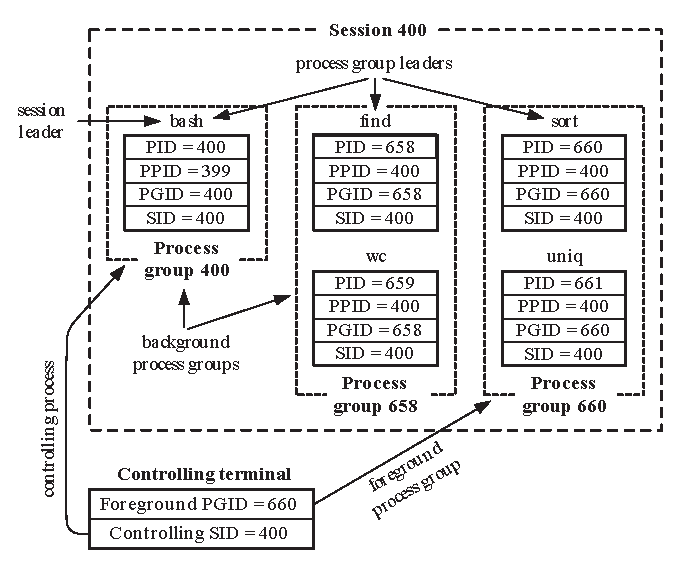
\includegraphics[width=0.65\textwidth]{fig/pgrp}
\end{center}
\caption{The controlling terminal has a session (set of process groups).
The foreground process group receives interactive control signals from
the terminal sent by the keyboard.  Only the foreground process group
may read from \texttt{stdin} and write to \texttt{stdout}; otherwise,
the process will receive the \texttt{SIGTTIN} or \texttt{SIGTTOU}
signal, respectively (which, by default stop the offending process).}
\label{fig:pgrp}
\end{figure}

Figure~\ref{fig:pgrp} shows a situation that can be easily reproduced
with the following commands:

\begin{minted}[bgcolor=lightgray]{text}
$ find . -name "*.c" | wc -l &
[1] 658 659
$ sort numbers.txt | uniq
\end{minted}

It is important to note that the shell (\texttt{bash} in this case)
places jobs in their own process groups immediately after
\texttt{fork()}ing.  This ensures that the shell is never a member of a
child process group.  This is important because, otherwise, interrupting
the foreground \texttt{sort number.txt | uniq} job in our example via
\ctrl{C} would send \texttt{SIGINT} to the \texttt{bash} (PID 400) along
with PIDs 660 and 661, which would kill not only the foreground process
group but our shell as well!  By putting jobs into their own process
groups, the shell protects itself from receiving such control signals
intended for the current foreground process group.

\pagebreak

Putting a process in a process group is easily accomplished:

\begin{minted}[bgcolor=lightgray]{c}
pid[t] = fork ();
setpgid (pid[t], pid[0]);

if (pid[t] == 0) {
    /* child stuff */
} else {
    /* parent stuff */
}
\end{minted}

Obviously, there is nuance to this.  First, keep in mind that passing a
zero to either argument of \texttt{setpgid()} has special meaning---the
following are all equivalent:

\begin{minted}[bgcolor=lightgray]{c}
setpgid (0, 0);
setpgid (getpid(), 0);
setpgid (getpid(), getpid());
\end{minted}

So, what we are doing in our \texttt{fork()} example above is to have
both the parent and the child attempt to put the child into a new
process group.  This is necessary because we don't know in what order
the scheduler will choose to execute these two processes after the
\texttt{fork()}.  Note, that there is no harm in placing a process into
a process group it is already a member of---simply nothing happens.  In
this way, regardless of which process (parent or child) gets schedule
first, the child will get kicked out of the parent's process group as
quickly as possible.



\section{Important \texttt{SIGCHLD} Details}

Keep in mind that when a child process changes its execution
\underline{state}, the parent process will receive a \texttt{SIGCHLD}
signal that must be waited on.  This may be caused by signals sent to
the \underline{child} such as \texttt{SIGTSTP}, \texttt{SIGCONT},
\texttt{SIGTERM}, \texttt{SIGKILL}, etc.  When the child receives one of
these signals (and changes state), the kernel subsequently sends the
parent a \texttt{SIGCHLD} signal so that it may act accordingly.  The
reason the kernel sent the \texttt{SIGCHLD} signal can be determined by
the parent process by investigating the \texttt{status} returned by
\texttt{waitpid}. This requires the use of the \texttt{WIF*} macros
detailed in the \texttt{waitpid man} page. For example:

\begin{minted}[bgcolor=lightgray]{c}
int status;
...
chld_pid = waitpid (-1, &status, WNOHANG | WUNTRACED | WCONTINUED)
...
if (WIFSTOPPED (status)) {
    /* child received SIGTSTP */
} else if (WIFCONTINUED (status)) {
    /* child received SIGCONT */
} else ...
\end{minted}

This is \underline{an} important opportunity for the parent to change
which process group is in the foreground---there are other important
opportunities as well, such as job creation.  This is accomplished by
calling \texttt{tcsetpgrp()} (read the \texttt{man} page).  Keep in mind
that when a foreground job completes, the shell's process group does
\underline{not} automatically get set to the foreground!  It is the
shell's responsibility to ensure that happens.



\section{Other Important Signals: \texttt{SIGTTIN} and \texttt{SIGTTOU}}

We have already discussed the fact that only the foreground process
group can read from \texttt{stdin} and write to \texttt{stdout}.  So...\
what happens when a process not in the foreground process group tries to
do one of these two activities?  Well, the process will receive
\texttt{SIGTTIN} if it tries to read from \texttt{stdin} and
\texttt{SIGTTOU} if it tries to write to \texttt{stdout}.  The default
handler for these signals stops the process.  This will obviously be a
big issue for your shell, which will potentially attempt to do both of
these things (e.g. the prompt!) while a foreground job is running.
\emph{Hint:} It may be smart for the shell to check if it is the
foreground process using \texttt{tcgetpgrp()} when in this scenario.
Keep in mind, a process can \underline{always} \texttt{pause()} until the
time is right...


\section{Process Groups are \underline{Not} Jobs (but they help!)}

In implementing your job system, you will find that you will not find
everything you need in process groups alone.  Job numbers, for example,
will have to be tracked by you; the name of the job (i.e. the command
entered at the prompt) will be too.  How will you know when a job is
done?  Better keep track of the PIDs of all your child processes so that
you can check every time one dies!  For simplicity, you only need to be
able to support a \textbf{\underline{maximum of 100}} simultaneously
managed jobs.  I suggest keeping an array of the following
\texttt{struct} to keep everything managed:

\begin{minted}[bgcolor=lightgray]{c}
typedef enum {
    STOPPED,
    TERM,
    BG,
    FG,
} JobStatus;

typedef struct {
    char* name;
    pid_t* pids;
    unsigned int  npids;
    pid_t pgid;
    JobStatus status;
} Job;
\end{minted}

I also suggest writing a small family of functions (i.e. an API) for
doing common job activities (e.g. adding, removing, killing, etc).  How
you actually end up doing this, however, is up to you.  If you want to
support $N$ simultaneously managed jobs, feel free to implement a linked
list of \texttt{Job} structures (but I think you already have enough to
deal with).  Just make sure what you design here works.


\section{Job Control Built-In Commands}

You will need to write four (4) built-in commands: \texttt{fg},
\texttt{bg}, \texttt{kill}, and \texttt{jobs}.  Unlike the
\texttt{which} command, I recommend running these job control commands
inside the shell process so that they have the ability to easily mutate
elements of the \texttt{Job} array.  Except for the \texttt{jobs}
command, all of these commands can accept a job number as an argument.
As you saw in the examples on Page 1, job numbers are decorated with a
leading percent (\texttt{\%}) character to indicate that the number that
follows is a job number.


\textbf{\underline{Built-in Command: fg}}

If no arguments are supplied, the following should be printed to the
screen and no job states are modified:

\begin{minted}[bgcolor=lightgray]{text}
Usage: fg %<job number>
\end{minted}

When a properly formatted job number (that exists) is supplied, the
corresponding job is moved to the foreground (and continued if
necessary).  If the supplied job number is not properly formatted or
corresponds to a job that does not exist, the following is printed to
\texttt{stdout}:

\begin{minted}[bgcolor=lightgray]{text}
pssh: invalid job number: [job number]
\end{minted}
where \texttt{[job number]} is the supplied (malformed or invalid) argument.

\pagebreak

\textbf{\underline{Built-in Command: bg}}

If no arguments are supplied, the following should be printed to the
screen and no job states are modified:

\begin{minted}[bgcolor=lightgray]{text}
Usage: bg %<job number>
\end{minted}

When a properly formatted job number (that exists) is supplied, the
corresponding job is continued but \underline{not} moved to the
foreground.  If the supplied job number is not properly formatted or
corresponds to a job that does not exist, the following is printed to
\texttt{stdout}:

\begin{minted}[bgcolor=lightgray]{text}
pssh: invalid job number: [job number]
\end{minted}
where \texttt{[job number]} is the supplied (malformed or invalid) argument.


\vspace{12pt}
\textbf{\underline{Built-in Command: kill}}

If no arguments are supplied, the following should be printed to the
screen and no job states are modified:

\begin{minted}[bgcolor=lightgray]{text}
Usage: kill [-s <signal>] <pid> | %<job> ...
\end{minted}

This means that a mixed list of PIDs and job numbers can be supplied to
the kill command, and the desired signal will be sent to each one
specified.  (The bar simply means the user can supply a pid
\underline{OR} a job number; the ellipsis just means the user can
supply as many of these as they like).  By default \texttt{SIGINT} is
sent.  If the optional \texttt{-s} argument is provided, then the
specified signal number is sent instead.

If an invalid job number is supplied, the following is printed to
\texttt{stdout}:

\begin{minted}[bgcolor=lightgray]{text}
pssh: invalid job number: [job number]
\end{minted}
where \texttt{[job number]} is the supplied job number.

If an invalid PID is supplied, the following is printed to
\texttt{stdout}:

\begin{minted}[bgcolor=lightgray]{text}
pssh: invalid pid: [pid number]
\end{minted}
where \texttt{[pid number]} is the supplied (malformed or invalid) argument.


\vspace{12pt}
\textbf{\underline{Built-in Command: jobs}}

This command takes no arguments.  All active jobs are simply printed to
\texttt{stdout} in the following format:

\begin{minted}[bgcolor=lightgray]{text}
[job number] + state     cmdline
\end{minted}

where \texttt{job number} is the job number, \texttt{state} is either
\texttt{stopped} or \texttt{running}, and \texttt{cmdline} is the
commmand line used to start the job.  Here is an example output showing
all possible states:

\begin{minted}[bgcolor=lightgray]{text}
[0] + stopped    foo | bar | baz
[2] + running    pi_computation
[3] + stopped    top &
\end{minted}


notice that it is absolutely possible for jobs to terminate in an order
different than they were started in (i.e. job 1 is already done)!
\textbf{The next job that is launched should therefore be job number 1
since it is the lowest available job number.}


\section{Providing Job Status Updates}

In addition to being able to run the built-in \texttt{jobs} command to
see if background jobs are stopped or running, the user should receive
feedback from your shell when:

\begin{enumerate}
    \item A foreground job is suspended via \ctrl{Z} (\texttt{SIGTSTP}).
         For example:

\begin{minted}[bgcolor=lightgray]{text}
$ ./my_program
Running...
^Z[1] + suspended      ./my_program
$ jobs
[0] + running    pi_computation
[1] + stopped    ./my_program
$
\end{minted}

    \item A stopped background job is continued (either via \texttt{bg}
            or by sending it \texttt{SIGCONT} directly using \texttt{kill}).
            For example:

\begin{minted}[bgcolor=lightgray]{text}
$ jobs
[0] + running    pi_computation
[1] + stopped    ./my_program
$ bg %1
[1] + continued  ./my_program
$ jobs
[0] + running    pi_computation
[1] + running    ./my_program
\end{minted}

    \item A background job completes or is terminated. For example:

\begin{minted}[bgcolor=lightgray]{text}
$ jobs
[0] + running    pi_computation
[1] + stopped    ./my_program
$ kill -s 9 %0
[0] + done       pi_computation
\end{minted}

    This ``done'' status message should \underline{not} be displayed when a
    foreground process completes/terminates---only background processes.

\end{enumerate}

\emph{Hint:} These messages to \texttt{stdout} are reports generated by
the shell when one of its child process groups changes status.
Consequently, these messages will be triggered within your shell's
\texttt{SIGCHLD} signal handler. Be careful though---some jobs will
consist of multiple processes!  If a job with 5 processes changes state,
you don't want the shell to report 5 status changes when the job is
continued, for example---you only want it to notify the user once that
the entire job has continued.

For the purposes of this exercise, feel free to put the necessary
\texttt{printf()} statements directly in your signal handler (although,
this is bad practice and should never be done in production code because
\texttt{printf()} is non-reentrant!).




\pagebreak

\section{Grading Rubric \& Convenient Feature Checklist}

When assessing the following table prior to submission (notice the fancy
check boxes for your benefit) please keep in
mind that although partial credit may be possible in extremely select
circumstances, it is not very likely. Do not halfway implement a feature
in a way that is completely non-functional, give up, and expect partial
credit.  Your features must actually work to receive credit.

\begin{longtable}[c]{@{}lll@{}}
\toprule\addlinespace
\begin{minipage}[t]{0.06\columnwidth}\raggedright
\end{minipage} & \begin{minipage}[t]{0.74\columnwidth}\raggedright
\textbf{Feature}
\end{minipage} & \begin{minipage}[t]{0.11\columnwidth}\raggedright
\textbf{Points}
\end{minipage}
\\\addlinespace\hline\addlinespace
\begin{minipage}[t]{0.06\columnwidth}\raggedright
\end{minipage} \checkbox & \begin{minipage}[t]{0.74\columnwidth}\raggedright
A process group is created for each new job. The PID of the first
process in the job is used as the PGID.
\end{minipage} & \begin{minipage}[t]{0.11\columnwidth}\raggedright
10
\end{minipage}
% \\\addlinespace\hline\addlinespace
% \begin{minipage}[t]{0.06\columnwidth}\raggedright
% \end{minipage} \checkbox & \begin{minipage}[t]{0.74\columnwidth}\raggedright
% Shell can handle jobs consisting of an arbitrary number of piplelined
% processes.
% \end{minipage} & \begin{minipage}[t]{0.11\columnwidth}\raggedright
% 10
% \end{minipage}
\\\addlinespace\hline\addlinespace
\begin{minipage}[t]{0.06\columnwidth}\raggedright
\end{minipage} \checkbox & \begin{minipage}[t]{0.74\columnwidth}\raggedright
A new job intended to run in the foreground is made the foreground
process group.
\end{minipage} & \begin{minipage}[t]{0.11\columnwidth}\raggedright
10
\end{minipage}
\\\addlinespace\hline\addlinespace
\begin{minipage}[t]{0.06\columnwidth}\raggedright
\end{minipage} \checkbox & \begin{minipage}[t]{0.74\columnwidth}\raggedright
A new job intended to run in the background is correctly setup and
launched in the background. Job number and associated PIDs are printed
to \texttt{stdout} by the shell as specified in the problem description.
\end{minipage} & \begin{minipage}[t]{0.11\columnwidth}\raggedright
10
\end{minipage}
\\\addlinespace\hline\addlinespace
\begin{minipage}[t]{0.06\columnwidth}\raggedright
\end{minipage} \checkbox & \begin{minipage}[t]{0.74\columnwidth}\raggedright
The shell process does not become stopped by SIGTTOU or SIGTTIN.
\end{minipage} & \begin{minipage}[t]{0.11\columnwidth}\raggedright
10
\end{minipage}
\\\addlinespace\hline\addlinespace
\begin{minipage}[t]{0.06\columnwidth}\raggedright
\end{minipage} \checkbox & \begin{minipage}[t]{0.74\columnwidth}\raggedright
The shell process properly waits on all child processes comprising jobs\\
(i.e. the shell does not generate a legion of zombie processes).
\end{minipage} & \begin{minipage}[t]{0.11\columnwidth}\raggedright
10
\end{minipage}
\\\addlinespace\hline\addlinespace
\begin{minipage}[t]{0.06\columnwidth}\raggedright
\end{minipage} \checkbox & \begin{minipage}[t]{0.74\columnwidth}\raggedright
A new background job is given the lowest available job number.
\end{minipage} & \begin{minipage}[t]{0.11\columnwidth}\raggedright
5
\end{minipage}
\\\addlinespace\hline\addlinespace
\begin{minipage}[t]{0.06\columnwidth}\raggedright
\end{minipage} \checkbox & \begin{minipage}[t]{0.74\columnwidth}\raggedright
Ctrl+Z (\texttt{SIGTSTP}) properly suspends the foreground job. The
\texttt{suspended} message specified in the project description is printed to
\texttt{stdout} by the shell informing the user accordingly. The shell
itself is not suspended and is moved to the foreground.
\end{minipage} & \begin{minipage}[t]{0.11\columnwidth}\raggedright
5
\end{minipage}
\\\addlinespace\hline\addlinespace
\begin{minipage}[t]{0.06\columnwidth}\raggedright
\end{minipage} \checkbox & \begin{minipage}[t]{0.74\columnwidth}\raggedright
Ctrl+C (\texttt{SIGINT}) properly terminates the foreground job. The
\texttt{done} message specified in the project description is \underline{NOT}
printed to \texttt{stdout} by the shell.  The shell itself is not
terminated and is moved to the foreground.
\end{minipage} & \begin{minipage}[t]{0.11\columnwidth}\raggedright
5
\end{minipage}
\\\addlinespace\hline\addlinespace
\begin{minipage}[t]{0.06\columnwidth}\raggedright
\end{minipage} \checkbox & \begin{minipage}[t]{0.74\columnwidth}\raggedright
Completed/terminated background jobs result in the shell printing the
\texttt{done} message specified in the project description to \texttt{stdout}.
The job is appropriately removed from the job management system.
\end{minipage} & \begin{minipage}[t]{0.11\columnwidth}\raggedright
5
\end{minipage}
\\\addlinespace\hline\addlinespace
\begin{minipage}[t]{0.06\columnwidth}\raggedright
\end{minipage} \checkbox & \begin{minipage}[t]{0.74\columnwidth}\raggedright
A job continued via either \texttt{bg} or \texttt{SIGCONT} properly
resumes running in the background and the \texttt{continued} message
specified in the project description is printed to \texttt{stdout} by
the shell.
\end{minipage} & \begin{minipage}[t]{0.11\columnwidth}\raggedright
5
\end{minipage}
\\\addlinespace\hline\addlinespace
\begin{minipage}[t]{0.06\columnwidth}\raggedright
\end{minipage} \checkbox & \begin{minipage}[t]{0.74\columnwidth}\raggedright
The \texttt{fg} built-in command functions as specified in the project
description.
\end{minipage} & \begin{minipage}[t]{0.11\columnwidth}\raggedright
5
\end{minipage}
\\\addlinespace\hline\addlinespace
\begin{minipage}[t]{0.06\columnwidth}\raggedright
\end{minipage} \checkbox & \begin{minipage}[t]{0.74\columnwidth}\raggedright
The \texttt{bg} built-in command functions as specified in the project
description.
\end{minipage} & \begin{minipage}[t]{0.11\columnwidth}\raggedright
5
\end{minipage}
\\\addlinespace\hline\addlinespace
\begin{minipage}[t]{0.06\columnwidth}\raggedright
\end{minipage} \checkbox & \begin{minipage}[t]{0.74\columnwidth}\raggedright
The \texttt{jobs} built-in command functions as specified in the project
description.
\end{minipage} & \begin{minipage}[t]{0.11\columnwidth}\raggedright
5
\end{minipage}
\\\addlinespace\hline\addlinespace
\begin{minipage}[t]{0.06\columnwidth}\raggedright
\end{minipage} \checkbox & \begin{minipage}[t]{0.74\columnwidth}\raggedright
The \texttt{kill} built-in command can send signals to specified PIDs.
\end{minipage} & \begin{minipage}[t]{0.11\columnwidth}\raggedright
5
\end{minipage}
\\\addlinespace\hline\addlinespace
\begin{minipage}[t]{0.06\columnwidth}\raggedright
\end{minipage} \checkbox & \begin{minipage}[t]{0.74\columnwidth}\raggedright
The \texttt{kill} built-in command can send signals to an entire process
group associated with a specified job number.
\end{minipage} & \begin{minipage}[t]{0.11\columnwidth}\raggedright
5
\end{minipage}
\\\addlinespace\hline\addlinespace
\begin{minipage}[t]{0.06\columnwidth}\raggedright
\end{minipage} \checkbox & \begin{minipage}[t]{0.74\columnwidth}\raggedright
The \texttt{kill} built-in command can send a user specified signal
number as specified by the optional \texttt{-s} parameter.
\end{minipage} & \begin{minipage}[t]{0.11\columnwidth}\raggedright
5
\end{minipage}
\\\addlinespace
\bottomrule
\end{longtable}


\pagebreak

\section{A Few Final Tips}

\begin{itemize}

    \item When calling \texttt{tcsetpgrp()}, you may find that the
        kernel is sending your shell \texttt{SIGTTOU} for apparently no
        reason.  This is generally handled by temporarily ignoring the
        \texttt{SIGTTOU} signal very briefly while performing the call.
        For example:

\begin{minted}[bgcolor=lightgray]{c}
    void (*old)(int);

    old = signal (SIGTTOU, SIG_IGN);
    tcsetpgrp (STDIN_FILENO, pgid);
    tcsetpgrp (STDOUT_FILENO, pgid);
    signal (SIGTTOU, old);
\end{minted}

    Do \underline{NOT} ignore \texttt{SIGTTOU} all the time,
    though---this will yield undesirable behavior.


\item Be careful not to accidentally close the \texttt{STDIN\_FILENO} or
    \texttt{STDOUT\_FILENO} file descriptors (i.e. 0 or 1) when setting
    up a job.  This is a great way to terminate your process
    prematurely.

\item The \texttt{kill()} function provided by \texttt{signal.h} has the
    in built ability to send a signal to all processes within a process
    group.  I suggest you read the \texttt{man} page:

\begin{minted}[bgcolor=lightgray]{text}
$ man 2 kill
\end{minted}

\item The following man pages also make for good reading and could prove
    to be extremely useful references:

\begin{minted}[bgcolor=lightgray]{text}
$ man 2 waitpid
$ man 2 signal
$ man 2 setpgid
$ man 3 tcgetpgrp
$ man 2 pause
\end{minted}

\end{itemize}


\section{Submitting Your Project}

Again, you will be building upon the codebase you developed for
\texttt{pssh} in Project 1.  Once you have implemented all of the
required features described in this document submit your code by doing
the following:

\begin{itemize}
    \item Run \texttt{make clean} in your source directory.  We must be
        able to build your shell from source and we don't want your
        precompiled executables or intermediate object files.
        \textbf{If your code does not at the very least compile, you
        will receive a zero.}

    \item Zip up your code:

\begin{minted}[bgcolor=lightgray]{bash}
jdoe@thanos:~/src$ ls -F
pssh/   pssh_v2/
jdoe@thanos:~/src$ zip -R jd619_pssh_v2.zip pssh_v2/*
\end{minted}

    \item Name your zip file \texttt{abc123\_pssh\_v2.zip}, where abc123
        is your Drexel ID.

    \item Upload your zip file using the Blackboard Learn submission
        link found on the course website.
\end{itemize}

\textbf{Failure to follow these simple steps will result in your project
not being graded.}

\begin{center}
    Now, have fun!
\end{center}


\begin{center}
\vspace{12pt}
\textbf{Due Thursday, Mar 8th \emph{before} midnight.}
\end{center}

\end{document}
